\documentclass[11pt, oneside]{article}   	% use "amsart" instead of "article" for AMSLaTeX format
\usepackage{geometry}                		% See geometry.pdf to learn the layout options. There are lots.
\geometry{letterpaper}                   		% ... or a4paper or a5paper or ...
%\geometry{landscape}                		% Activate for rotated page geometry
%\usepackage[parfill]{parskip}    		% Activate to begin paragraphs with an empty line rather than an indent
\usepackage{graphicx}				% Use pdf, png, jpg, or eps§ with pdflatex; use eps in DVI mode
								% TeX will automatically convert eps --> pdf in pdflatex
\usepackage{amssymb}

% % listings begin
\usepackage{listings}
% \providecommand{\GitRemote}{}
% \providecommand{\GitIdentifier}{master}
% \providecommand{\GitCheckout}[2][\GitIdentifier]{%
% % #1 being the version/branch
% % #2 being the file
% | \string"git archive --remote=\GitRemote #1 \detokenize{#2} 2>/dev/null | tar --extract --file - --to-stdout \string"%
% }
% % listings end

\usepackage{tikz}
\usetikzlibrary{positioning}
\usepackage{mathtools}

%SetFonts

%SetFonts

% External dependencies
\usepackage{pagecolor}
\input{../../../../include/hmath_descendant.tex}
% \input{https://github.com/hovey/include/blob/a9bf6db0394b5ba19e69653519a96c10eeb1e133/hmath_descendant.tex}
% https://tex.stackexchange.com/questions/500463/using-listinputlisting-to-include-a-specific-git-commit
% https://git-scm.com/docs/git-archive
% https://tex.stackexchange.com/questions/500463/using-listinputlisting-to-include-a-specific-git-commit

\title{Laplace Smoothing}
\author{C.B.~Hovey}
%\date{} % Activate to display a given date or n date

\begin{document}
\maketitle
%\section{}
%\subsection{}

% renewcommand{\GitRemote}{ssh://git@trac.sagemath.org/sage.git}
% \lstinputlisting{\GitCheckout{src/sage/coding/goppa.py}}
% \renewcommand{\GitRemote}{ssh://git@github.com:hovey/include.git}
% \lstinputlisting{\GitCheckout{hovey/include/hmath_descendant.tex}}

% \lstinputlisting{|\string"git archive --remote=ssh://git@server/repo.git VERSION path/to/file 2>/dev/null | tar --extract --file - --to-stdout\string"}
% \lstinputlisting{|\string"git archive --remote=ssh://git@github.com:hovey/include.git v0.0.1 hmath_descendant.tex 2>/dev/null | tar --extract --file hmath_descendant.tex --to-stdout\string"}
% \lstinputlisting{|\string"git archive --remote=https://git@github.com/hovey/include.git include/hmath_descendant.tex 2>/dev/null | tar --extract --file hmath_descendant.tex --to-stdout\string"}
% \lstinputlisting{|\string"git archive --remote=https://git@github.com/hovey/include.git v0.0.1 include/hmath_descendant.tex 2>/dev/null | tar --extract --file - --to-stdout\string"}


Let the subject node have a current configuration located at
point $\vp \in \realnsd$ have coordinates relative to origin $O$
of
$(x)$ in 1D,
$(x, y)$ in 2D,
and $(x, y, z)$ in 3D.
The subject point connects to $n$ neighbor points
$\vq_i$ for $i \in [1, n]$ though $n$ edges.
In Fig.~\ref{fig:node_p}, for example, the point $\vp$ connects for four
neighbors.

\begin{figure}[htb]
  \begin{center}

    \begin{tikzpicture}
      \draw[lightgray, thin] (0,0) -- (1,0);  % x-axis
      \draw[lightgray, thin] (0,0) -- (0,1); % y-axis
      \draw[lightgray, thin] (0,0) -- (-0.55, -0.55); % z-axis
      \draw[green, thick] [-stealth](0,0) -- (4,4);  % center, pbar
      \draw[blue, thick] [-stealth](0,0) -- (2.5,6);  % p
      % \draw[dashed, red, thick] [-stealth](4,4) -- (2.5,6);  % g
      \draw[dashed, red, thick] [-stealth](2.5,6) -- (4,4);  % Dp

      \draw[dotted, blue, thick] (4,8) -- (2.5,6);  % p to north
      \draw[dotted, blue, thick] (0,4) -- (2.5,6);  % p to west
      \draw[dotted, blue, thick] (4,0) -- (2.5,6);  % p to south
      \draw[dotted, blue, thick] (8,4) -- (2.5,6);  % p to east

      \filldraw[black] (0,0) circle (2pt) node[anchor=east]{$O$};
      % \filldraw[black] (4,4) circle (2pt) node[anchor=south]{$\bar{\vp}$};
      \filldraw[black] (4,4) circle (2pt) node[anchor=south]{$\bar{\vq}$};
      \filldraw[black] (2.5,6) circle (2pt) node[anchor=south]{$\vp$};
      % \filldraw[black] (3.25,5) circle (0pt) node[anchor=south]{$\vg$};
      \filldraw[black] (3.25,5) circle (0pt) node[anchor=south]{$\Delta \vp$};
      \filldraw[black] (4,8) circle (2pt) node[anchor=south]{$\vq_i$};
      \filldraw[black] (0,4) circle (2pt) node[anchor=south]{$\vq_{i+1}$};
      \filldraw[black] (4,0) circle (2pt) node[anchor=south]{$\vq_{n-1}$};
      \filldraw[black] (8,4) circle (2pt) node[anchor=south]{$\vq_n$};
    \end{tikzpicture}

  \end{center}

  \caption{Subject node with current configuration at $\vp$ with edge
  connections (dotted lines)
  to neighbor nodes $\vq_i$
  with $i \in [1, n]$ (without loss of generality,
  the specific example of $n = 4$ is shown).
  The average position of all neighbors of $\vp$
  is denoted $\bar{\vq}$, and the gap $\Delta \vp$ (dashed line)
  originates at $\vp$ and terminates at $\bar{\vq}$.}
\label{fig:node_p} % label must come after caption
\end{figure}
Let $\bar{\vq}$ denote the average position of all neighbors of $\vp$ and be
defined as
\be
  \bar{\vq} \coloneqq \frac{1}{n} \sum_{i=1}^n \vq_i.
\ee
Let the gap vector $\Delta \vp$ be defined as originating at $\vp$ and
terminating at $\bar{\vq}$, such that
\be
 \Delta \vp \coloneqq \bar{\vq} - \vp, \;\;\; \mbox{since} \;\;\; \vp + \Delta \vp = \bar{\vq}.
\ee
Let $\lambda \in \realplus \subset (0, 1)$ be a scaling factor for the
gap $\Delta \vp$.  Then we seek to iteratively update the position of $\vp^{(k)}$ at the
$k^{\mbox{\tiny th}}$ iteration by an amount $\lambda \Delta \vp^{(k)}$ to $\vp^{(k+1)}$ as
\begin{align}
  \vp^{(k+1)} & \coloneqq \vp^{(k)} + \lambda \Delta \vp^{(k)}, \hspace{0.5cm} \mbox{since} \\
  \bar{\vq} & = \vp + \Delta \vp \hspace{0.5cm} \mbox{when } \lambda = 1.
\end{align}
We typically select $\lambda < 1$ to avoid overshoot of the update.  Following
are two iterations for $\lambda = 0.1$ and initial positions $\vp = 1.5$ and
$\bar{\vq} = 0.5$ (given two neighbors, one at 0.0 and one at 1.0, that
never move), a simple 1D example:

\begin{table}[htb]
  \caption{Two iteration update of a 1D example.}
  \label{tab:update_example} % label must come after caption
  \centering
  \begin{tabular}{c|c|c|l|l}
    $k$ & $\bar{\vq}$ & $\vp^{(k)}$ & $\Delta \vp^{(k)} = \bar{\vq} - \vp^{(k)}$ & $\lambda \Delta \vp^{(k)}$ \\
   \hline
   \hline
   0 & 0.5 & 1.5 & -1.0 & -0.1 \\
   1 & 0.5 & 1.5 - 0.1 = 1.4 & -0.9 & -0.09 \\
   2 & 0.5 & 1.4 - 0.09 = 1.31 & -0.81 & -0.081
  \end{tabular}
\end{table}

\begin{figure}[htb]
  \begin{center}

    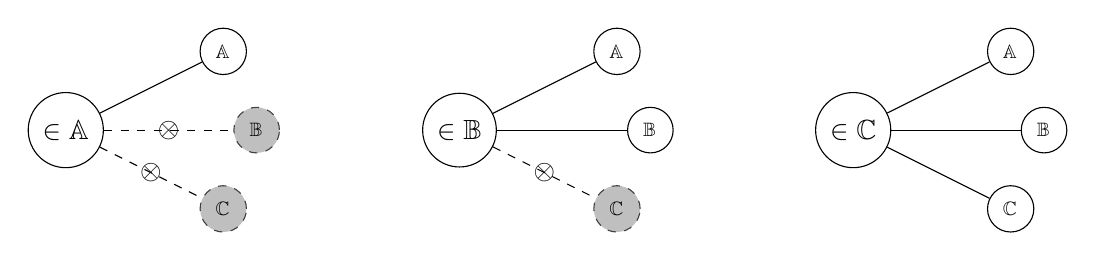
\begin{tikzpicture}
      \node[shape=circle,draw=black] (a) at (-6,0) {$\vp \in \mathbb{A}$};
      \node[shape=circle,draw=black] (b) at (-4,1) {$\vq_{\mathbb{A}}$};
      \node[shape=circle,draw=darkgray, dashed, fill=lightgray] (c) at (-3.576,0) {$\vq_{\mathbb{B}}$};
      \node[shape=circle,draw=darkgray, dashed, fill=lightgray] (d) at (-4,-1) {$\vq_{\mathbb{C}}$};

      \node[shape=circle,draw=black] (e) at (-1,0) {$\vp \in \mathbb{B}$};
      \node[shape=circle,draw=black] (f) at (1,1) {$\vq_{\mathbb{A}}$};
      \node[shape=circle,draw=black] (g) at (1.424,0) {$\vq_{\mathbb{B}}$};
      \node[shape=circle,draw=darkgray, dashed, fill=lightgray] (h) at (1,-1) {$\vq_{\mathbb{C}}$};

      \node[shape=circle,draw=black] (i) at (4,0) {$\vp \in \mathbb{C}$};
      \node[shape=circle,draw=black] (j) at (6,1) {$\vq_{\mathbb{A}}$};
      \node[shape=circle,draw=black] (k) at (6.424,0) {$\vq_{\mathbb{B}}$};
      \node[shape=circle,draw=black] (l) at (6,-1) {$\vq_{\mathbb{C}}$};

      \path (a) edge (b);
      \path [dashed](a) edge node[align=center] {$\otimes$} (c);
      \path [dashed](a) edge node[align=center] {$\otimes$} (d);

      \path (e) edge (f);
      \path (e) edge (g);
      \path [dashed](e) edge node[align=center] {$\otimes$} (h);

      \path (i) edge (j);
      \path (i) edge (k);
      \path (i) edge (l);
    \end{tikzpicture}

  \end{center}

  \caption{Hierarchical classification of nodes based on categories of surface $\mathbb{A}$, interface $\mathbb{B}$, and interior $\mathbb{C}$.}
\label{fig:hierarchy} % label must come after caption
\end{figure}

% \begin{figure}[htb]
%   \begin{center}
%
%     \begin{tikzpicture}[
%     roundnode/.style={circle, draw=green!60, fill=green!5, very thick, minimum size=7mm},
%     squarednode/.style={rectangle, draw=red!60, fill=red!5, very thick, minimum size=5mm},
%     ]
%     %Nodes
%     \node[roundnode] (center)                  {$\vp$};
%     \node[roundnode] (upper) [above=of center] {$\vq_1$};
%     \node[roundnode] (left)  [left=of center]  {$\vq_2$};
%     \node[roundnode] (lower) [below=of center] {$\vq_i$};
%     \node[roundnode] (right) [right=of center] {$\vq_{n}$};
%
%     %Lines
%     \draw[-] (center.north) -- (upper.south);
%     \draw[-] (center.west) -- (left.east);
%     \draw[-] (center.south) -- (lower.north);
%     \draw[-] (center.east) -- (right.west);
%     % \draw[-] (upper.south) -- (center.north);
%     % \draw[-] (right.south) .. controls +(down:7mm) and +(right:7mm) .. (lower.east);
%     \end{tikzpicture}
%
%   \end{center}
%
%   \caption{Subject node $\vp$ with edge connections to neighbor nodes $\vq_i$ with $i \in [1, n]$.}
% \label{fig:single_node} % label must come after caption
% \end{figure}





\end{document}
